%###############################################################################
%# N1 - Manual - Memory map                                                    #
%###############################################################################
%#    Copyright 2018 - 2019 Dirk Heisswolf                                     #
%#    This file is part of the N1 project.                                     #
%#                                                                             #
%#    N1 is free software: you can redistribute it and/or modify               #
%#    it under the terms of the GNU General Public License as published by     #
%#    the Free Software Foundation, either version 3 of the License, or        #
%#    (at your option) any later version.                                      #
%#                                                                             #
%#    N1 is distributed in the hope that it will be useful,                    #
%#    but WITHOUT ANY WARRANTY; without even the implied warranty of           #
%#    MERCHANTABILITY or FITNESS FOR A PARTICULAR PURPOSE.  See the            #
%#    GNU General Public License for more details.                             #
%#                                                                             #
%#    You should have received a copy of the GNU General Public License        #
%#    along with N1.  If not, see <http://www.gnu.org/licenses/>.              #
%###############################################################################
%# Version History:                                                            #
%#   April 26, 2019                                                         #
%#      - Initial release                                                      #
%###############################################################################

\section{Memory Map}
\label{memmap}

The N1's configuration options support a variety of layouts for the system's 128KB
memory space.
However if the memory layout is not constrained by the integrating system, the
two memory maps as shown in \figref{memmap:recommendations} are recommended.

\begin{figure}[!htb]
  %\begin{center}
  \makebox[\textwidth][c]{
    \scalebox{1} {
      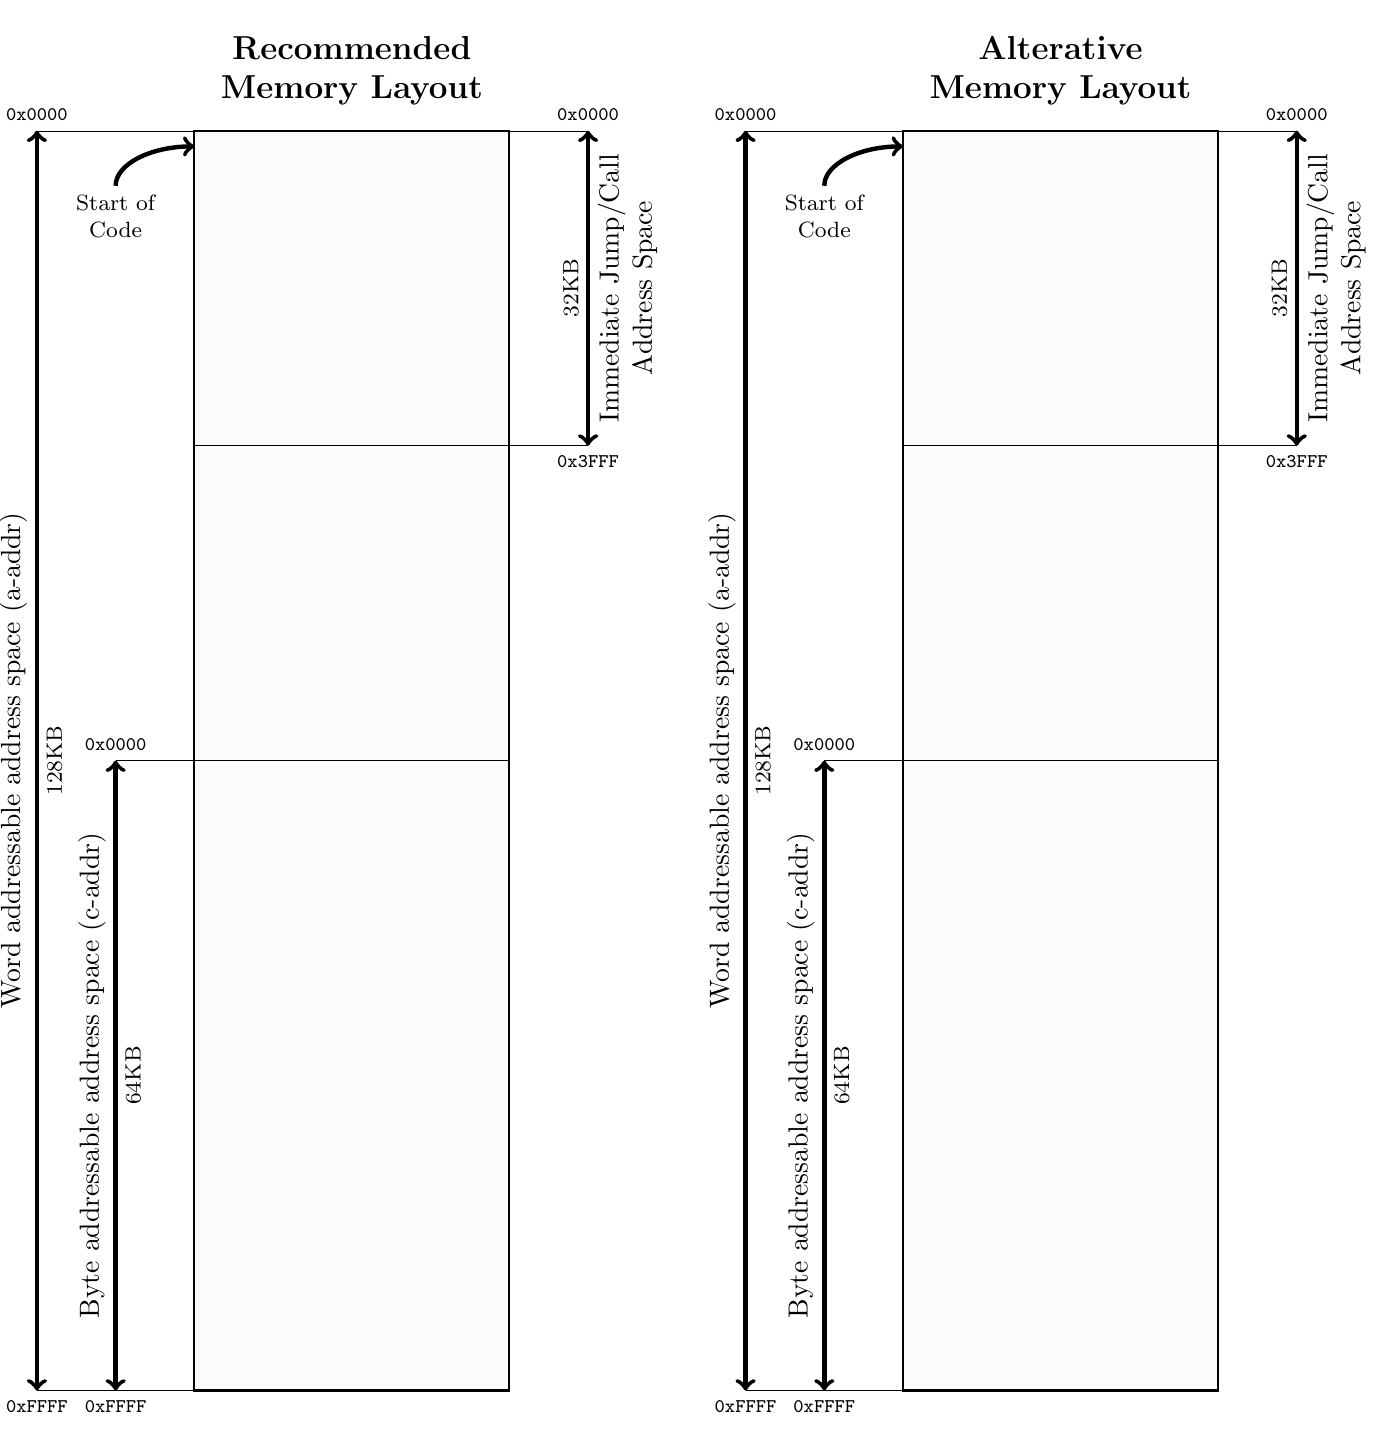
\begin{tikzpicture}
      
        %Framework
        \newsavebox{\memframe}
        \savebox{\memframe}{

          %Memory
          \draw [thick, fill=gray!3] (2,0) rectangle (6,16);

          %Word addressable space
            \draw [ultra thick, <->] (0,0)  -- (0,16);
            \draw [ultra thin]       (0,0)  -- (6,0);
            \draw [ultra thin]       (0,16) -- (6,16);

            \node [above] at (0,16) {
              \scriptsize{\texttt{0x0000}}};
            \node [below] at (0,0) {
              \scriptsize{\texttt{0xFFFF}}};
            \node [below,rotate=90] at (0,8) {
                  \footnotesize{128KB}
            };
            \node [above,rotate=90] at (0,8) {
                  Word addressable address space
                 (a-addr)
            };

          %Byte addressable space
            \draw [ultra thick, <->] (1,0) -- (1,8);
            \draw [ultra thin]       (1,8) -- (6,8);
            \node [above] at (1,8) {
              \scriptsize{\texttt{0x0000}}};
            \node [below] at (1,0) {
              \scriptsize{\texttt{0xFFFF}}};
            \node [below,rotate=90] at (1,4) {
              \footnotesize{64KB}
            };
            \node [above,rotate=90] at (1,4) {
                  Byte addressable address space
                 (c-addr)
             };

            %Immediate jump or call addressing
            \draw [ultra thick, <->] (7,12) -- (7,16);
            \draw [ultra thin]       (2,12) -- (7,12);
            \draw [ultra thin]       (2,16) -- (7,16);
            \node [above] at (7,16) {
              \scriptsize{\texttt{0x0000}}};
            \node [below] at (7,12) {
              \scriptsize{\texttt{0x3FFF}}};
            \node [above,rotate=90] at (7,14) {
              \footnotesize{32KB}
            };
            \node [below,rotate=90] at (7,14) {
              \begin{minipage}[c]{14em}
                \center
                  Immediate
                  Jump/Call \\
                  Address Space
            \end{minipage}};

            %Start of code
            \draw [ultra thick, <-] (2,15.8) arc (90:180:1 and .5);
            \node [below] at (1,15.3) {
              \begin{minipage}[c]{14em}
                \center
                \footnotesize{Start of \\ Code}
            \end{minipage}};
            
            
        };

        %First recommendation
        \begin{scope}[shift={(-8,0)}]
          \node [above] at (4,16.2) {
            \begin{minipage}[c]{20em}
              \center
              \large{\textbf{Recommended\\Memory Layout}}
            \end{minipage}};          
          \node at (0,0) {\usebox{\memframe}};
        \end{scope}

        %Second recommendation
        \begin{scope}[shift={(1,0)}]
          \node [above] at (4,16.2) {
            \begin{minipage}[c]{20em}
              \center
              \large{\textbf{Alterative\\Memory Layout}}
            \end{minipage}};
          \node at (0,0) {\usebox{\memframe}};
        \end{scope}
        
      \end{tikzpicture}
    }
  }
  \caption{Memory Layout Recommendations}
  \label{memmap:recommendations}
  %\end{center}
\end{figure}
